\chapter{Grundlagen} \label{cha:Grundlagen}

Nicht vergessen, dass Überschriften nicht aufeinander folgen dürfen\ldots


\section{Section} \label{sec:Section2}

Label Beispiel (vgl. \cref{sec:Section})

% a example citation
\cite{Kammeyer}

% using glossary entries. symbols and acronyms are defined in backmatter/symbols_and_acronyms
\gls{ieee}

\gls{ieee}

\gls{abc}

\gls{led}

\glssymbol{angstrom} \gls{angstrom}

\gls{led}

% example equation
The ratio of the circumference of a circle to its diameter is given by \gls{pi}:
\begin{equation}
\glssymbol{pi} = \frac{C}{d} \cdot \glssymbol{ohm}
\end{equation}

\begin{equation}
U = R \cdot I
\end{equation}


% example figure
\begin{figure}[htbp]
\centering
\begin{circuitikz}[european inductors, european resistors]
\draw [help lines] (0,0) grid (8,4);
\draw
(0,0) node[anchor=east]{} to [short, o-](8,0)
(0,4) node[anchor=east]{} to [short,i=$\textbf{i}_s^s$, o-](1,4)
to[R,l=$\text{R}_{\text{s}}$](3,4)
to[L,l=$\text{L}_{\text{sl}}$](5,4)
to[L,l=$\text{L}_{\text{rl}}$,i>=$\textbf{i}_r^s$](8,4)
to[R,l=${\text{R}'}_{\text{r}}$](8,2) -- (8,1.5) (8,1) -- (8,0) (5,4)
to[L,i>^=$\textbf{i}_m^s$,l=$\text{L}_{\text{m}}$,-*](5,0)
;\draw
(8,1) node[fill=white,shape=circle,minimum size=30,draw,
label={[xshift=0.5cm, yshift=-0.2cm]\textbf{+}},
label={[xshift=1.2cm, yshift=-0.8cm]j$\omega_r\mathbf{\varPsi}_r^s$}]{}
;
\end{circuitikz}
\captionbelow{Dynamic equivalent circuit for an induction machine}
\label{fig:dyneqmodel}
\end{figure}

% some siunitx examples

\num{12345,67890} \\
\num{1+-2i} \\
\num{.3e45} \\
\num{1.654 x 2.34 x 3.430}

\si{kg.m.s^{-1}} \\
\si{\kilogram\metre\per\second} \\
\si[per-mode=symbol]
{\kilogram\metre\per\second} \\
\si[per-mode=symbol]
{\kilogram\metre\per\ampere\per\second}

\numlist{10;20;30}
\SIlist{0.13;0.67;0.80}{\milli\metre} \\
\numrange{10}{20} \\
\SIrange{0.13}{0.67}{\milli\metre}

\newglossaryentry{c0}{type=symbol,name=c0,symbol={\si{\clight}},description={\SI[scientific-notation = engineering]{299792458}{\meter\per\second}, speed of light}}

\glssymbol{c0}
\newpage
\section{Hello newpage}

\begin{table}[htb]
\centering
\captionabove{Dies ist nur eine Beispieltabelle}
\label{tbl:beispiel}
\begin{tabular}{l|lll}
Dies & ist & ein & Beispiel.\\\hline
Bitte & lassen & Sie & den \\
Inhalt & dieser & Tabelle & unbeachtet.
\end{tabular}
\end{table}

Booktabs Tabellenbeispiel

\begin{table}[htb]
	\captionabove[IEEE~802.11a und IEEE~802.11p PHY-Parameter im Vergleich]{IEEE~802.11a und IEEE~802.11p PHY-Parameter im Vergleich\,\cite{IEEE2012}}
	\label{tbl:params}
	\footnotesize
	\centering
	\rowcolors{2}{white}{gray!25}	%TUgreen!25
	\begin{tabular}{m{5cm}*{2}{c}}	%p{}m{}b{}clr
	\toprule
	\textbf{Parameter} & \textbf{IEEE~802.11a} & \textbf{IEEE~802.11p} \\
	\midrule
	Kanalbandbreite $B$ & \SI{20}{\mega\hertz} & \SI{10}{\mega\hertz} \\
	Maximale Sendeleistung $P_\text{S}$ & \SI{20}{\dBm} & \SI{33}{\dBm} \\
	Datenrate [\si{\mega\bit\per\second}] & 6, 9, 12, 18, 24, 36, 48, 54 & 3, 4.5, 6, 9, 12, 18, 24, 27 \\
	Modulationen & BPSK, QPSK, 16-QAM, 64-QAM & BPSK, QPSK, 16-QAM, 64-QAM \\
	Coderaten & \num{1 / 2}, \num{2 / 3}, \num{3 / 4} & \num{1 / 2}, \num{2 / 3}, \num{3 / 4} \\
	Anzahl Datensubträger ($N_{\text{SD}}$) & 48 & 48 \\
	Anzahl Pilotsubträger ($N_{\text{SP}}$) & 4 & 4 \\
	Gesamtanzahl Subträger ($N_{\text{ST}}$) & 52 ($N_{\text{SD}} + N_{\text{SP}}$) & 52 ($N_{\text{SD}} + N_{\text{SP}}$) \\
	Subträgerabstand ($\Delta f$) & \SI{312.50}{\kilo\hertz} ($\frac{\SI{20}{\mega\hertz}}{\num{64}}$) & \SI{156.25}{\kilo\hertz} ($\frac{\SI{10}{\mega\hertz}}{\num{64}}$) \\
	Dauer (Inverse) Fast Fourier\-trans\-for\-ma\-tion ($T_{\text{FFT}}$) & \SI{3.2}{\micro\s} ($\frac{1}{\Delta f}$) & \SI{6.4}{\micro\s} ($\frac{1}{\Delta f}$)\\
	Dauer Guard Interval $T_{\text{GI}}$ & \SI{0.8}{\micro\s} ($\frac{T_{\text{FFT}}}{4}$) & \SI{1.6}{\micro\s} ($\frac{T_{\text{FFT}}}{4}$) \\
	Dauer Training Symbol GI $T_{\text{GI2}}$ & \SI{1.6}{\micro\s} ($\frac{T_{\text{FFT}}}{2}$) & \SI{3.2}{\micro\s} ($\frac{T_{\text{FFT}}}{2}$) \\
	Symbol Interval $T_{\text{SYM}}$ & \SI{4}{\micro\s} ($T_{\text{GI}} + T_{\text{FFT}}$) & \SI{8}{\micro\s} ($T_{\text{GI}} + T_{\text{FFT}}$) \\
	Präambellänge $T_{\text{Preamble}}$ & \SI{16}{\micro\s} & \SI{32}{\micro\s} \\
	\bottomrule
	\end{tabular}
\end{table}

Quellcodebeispiel mit Seitenumbruch

\singlespacing
\begin{matlab}[firstnumber=1, name=MATLABCodeBeispiel, caption={MATLAB Code Beispiel}, label={lst:MATLABCodeBeispiel}]
%instrreset
clear all
oldobjs=instrfind;
if ~isempty(oldobjs)
disp('Cleaning up ...')
delete(oldobjs);
clear oldobjs;
end

close all;
clear all;


samprate = 65833332;    % 65833333 disables HF Filter  % Sample Rate
trigger = 'IMM';        % Trigger setting. IMM, IFP or EXT
nosamples = 8000;       % No. Captured IQ Sample Pairs. Max 2 MB also 262144 IQ/Samples
dispupdate = 'On';      % Analyser Display On or Off

freq_center = 2412e6;
channel_bw = 20e6;
power_level = -40; % [dBm]
\end{matlab}
\onehalfspacing

\begin{figure}[htbp]
	\centering
	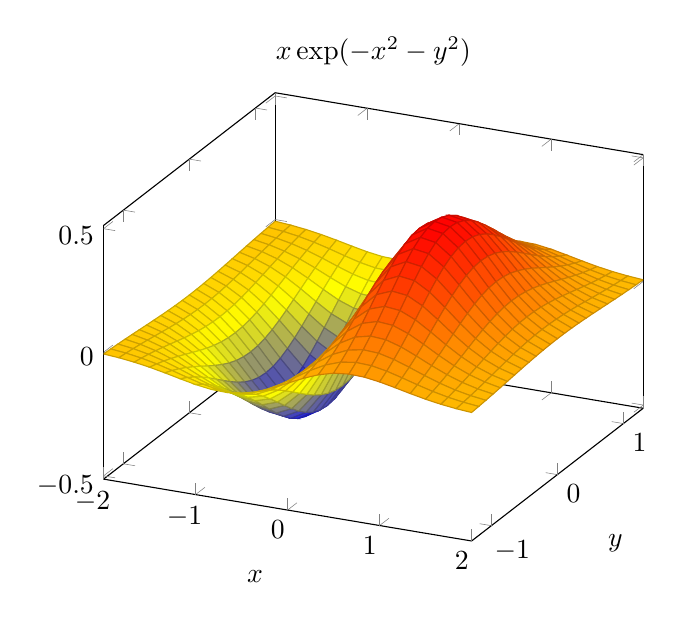
\begin{tikzpicture}
		\begin{axis}[
		title={$x \exp(-x^2-y^2)$},
		xlabel=$x$, ylabel=$y$,
		]
		\addplot3[
		surf,				%contour gnuplot		% for gnuplot test
		domain=-2:2,
		domain y=-1.3:1.3,
		]
		{exp(-x^2-y^2)*x};
		\end{axis}
	\end{tikzpicture}
	\captionbelow{Plot of a Math Expression}
	\label{fig:mathplot}
\end{figure}